%  sample eprint article in LaTeX           --- M. Peskin, 9/7/00
%  modified for CTD2023, ctd2023-loc@l2it.in2p3.fr
%  This file is part of a tar file, which can be downloaded from the CTD2023 indico site. 
%  indico.cern.ch/e/CTD2023
%
\documentclass[10pt, paper=a4, UKenglish]{article}
%
%%%%%%%%%%%%%%%%%%%%%%%%%%%%%%%%%%%%%%%%%%%%%%%%%%%%%%%%%%%%%%%%%%%%%%%%%%%%
%   document style macros
%%%%%%%%%%%%%%%%%%%%%%%%%%%%%%%%%%%%%%%%%%%%%%%%%%%%%%%%%%%%%%%%%%%%%%%%%%%%
\def\Title#1{\begin{center} {\Large #1 } \end{center}}
\def\Author#1{\begin{center}{ \sc #1} \end{center}}
\def\Address#1{\begin{center}{ \it #1} \end{center}}
\def\andauth{\begin{center}{and} \end{center}}
\def\submit#1{\begin{center}Submitted to {\sl #1} \end{center}}
\newcommand\pubblock{\rightline{\begin{tabular}{l} Proceedings of the CTD 2023\\ \pubnumber\\
         \pubdate  \end{tabular}}}

\newenvironment{Abstract}{\begin{quotation} \begin{center} 
             \large ABSTRACT \end{center}\bigskip 
      \begin{center}\begin{large}}{\end{large}\end{center} \end{quotation}}

\newenvironment{Presented}{\begin{quotation} \begin{center} 
             PRESENTED AT\end{center}\bigskip 
      \begin{center}\begin{large}}{\end{large}\end{center} \end{quotation}}

\def\Acknowledgements{\bigskip  \bigskip \begin{center} \begin{large}
      \bf ACKNOWLEDGEMENTS \end{large}\end{center}}

%%%%%%%%%%%%%%%%%%%%%%%%%%%%%%%%%%%%%%%%%%%%%%%%%%%%%%%%%%%%%%%%%%%%%%%%%%%% 
%  personal abbreviations and macros
%    the following package contains macros used in this document:
\input econfmacros.tex
%%%%%%%%%%%%%%%%%%%%%%%%%%%%%%%%%%%%%%%%%%%%%%%%%%%%%%%%%%%%%%%%%%%%%%%%%%%

\textwidth=6.5in
\textheight=8.75in
\hoffset=-0.85in
\voffset=-0.6in

%%  DO NOT CHANGE anything above.

% include packages you will need
\usepackage{color}
\usepackage[dvipsnames]{xcolor}
\usepackage{lineno}
\usepackage{subfig}
\usepackage{hyperref}
\usepackage{graphicx}
\usepackage[style=numeric,backend=bibtex,natbib=true]{biblatex}
\usepackage{amsmath}
\usepackage{overpic}
\addbibresource{bibliography.bib}

%%%%%%%%%%%%%%%%%%%%%%%%%%%%%%%%%%%%%%%%%%%%%%%%%%%%%%%%%%%%%%%%%%%%
% basic data for the eprint:
%%%%%%%%%%%%%%%%%%%%%%%%%%%%%%%%%%%%%%%%%%%%%%%%%%%%%%%%%%%%%%%%%%%%

%% preprint number data:
% Please replace XX by your contribution number in indico (a number between 01 to 62)
\newcommand\pubnumber{PROC-CTD2023-49}

%% date
\newcommand\pubdate{\today}

%%  Affiliation
\def\affiliation{
On behalf of the Acts and ODD community \\
Fakultät für Physik, TU Wien, Austira \\
CERN}

%% Acknowledge the support
\def\support{\footnote{Work supported by CERN}}

%%%%%%%%%%%%%%%%%%%%%%%%%%%%%%%%%%%%%%%%%%%%%%%%%%%%%%%%%%%%%%%%%%%%%%%%%%%% 

\newcommand{\conference}{Connecting the Dots Workshop (CTD 2023)\\
October 10-13, 2023}

\usepackage{fancyhdr}
\pagestyle{fancy}
\definecolor{mygrey}{RGB}{105,105,105}
\fancyhf{} % sets both header and footer to nothing
\renewcommand{\headrulewidth}{0pt}
% \fancyhead[R]{\fontsize{8}{9} \color{mygrey} \selectfont  CTD 2022 \\}
\fancyhead[C]{\fontsize{7}{8} \color{mygrey} \selectfont Connecting
  the Dots. October 10-13, 2023\\}
\fancyfoot[C]{\thepage}

%%%%%%%%%%%%%%%%%%%%%%%%%%%%%%%%%%%%%%%%%%%%%%%%%%%%%%%%%%%%%%%%%%%%

\begin{document}

% uncomment the following line for adding line numbers
% \linenumbers

% large size for the first page
\large
\begin{titlepage}
\pubblock

%% Change the title, name, abstract
%% Title 
\vfill
\Title{Reconstruction performance with ACTS and the Open Data Detector}
\vfill

%  if you need to add the support use this, fill the \support definition above. 
%  \Author{FIRSTNAME LASTNAME \support}
\Author{Pierfrancesco Butti\textsuperscript{1}, Noemi Calace\textsuperscript{2}, Paul Gessinger-Befurt\textsuperscript{2}, Benjamin Huth\textsuperscript{3}, Andreas Salzburger\textsuperscript{2}, Andreas Stefl\textsuperscript{2,4}}
\Address{SLAC (1), CERN (2), Universität Regensburg (3), TU Wien (4)}
\vfill

\begin{Abstract}
Over the last years, the ACTS software has matured in functionality and performance while at the same time the Open Data Detector (ODD), a revision and evolution of the TrackML detector, has been established. Together they form a foundation for track reconstruction algorithms research and performance evaluation, including 4D tracking with time information. In this contribution we present the performance of the reconstruction chain for silicon based detectors implemented in ACTS using both particle gun and $t\overline{t}$ with variable pileup. This serves as a validation for both the ODD geometry and the ACTS reconstruction algorithms. At the same time it is a reference for experiments looking into ACTS reconstruction performance. Additionally, we use it to validate the ACTS intrinsic fast track simulation (ActsFatras) and present a coherent continuous integration testing suite to monitor performance changes over time.
\end{Abstract}

\vfill

% DO NOT CHANGE!!!
\begin{Presented}
\conference
\end{Presented}
\vfill
\end{titlepage}
\def\thefootnote{\fnsymbol{footnote}}
\setcounter{footnote}{0}
%

% normal size for the rest
\normalsize 

%% Your paper should be entered below. 

\section{Introduction}
\label{intro}

ACTS is a common tracking software which provides various reconstruction algorithms for charged particles in particle physics experiments\cite{acts}. Its key objectives are to be experiment independent, thread-safe, modular and composable, written in modern C++, and to act as a tracking algorithm R\&D platform.

In order to develop, validate and evaluate the experiment independent tracking algorithms, one needs a detector geometry which is preferably open for the public and free of license. The TackML challenge showed that such an environment opens up new channels of knowledge transfer and collaboration.

The Open Data Detector (ODD) is an evolution of the TrackML detector with a more realistic material budget and full simulation support with Geant4. It is an (HL-)LHC-like full silicon prototype inner detector based on DD4hep and consists of 3 sub detectors: Pixel, Short Strips, and Long Strips. The ODD can be extended with calorimeters\cite{odd_chep} and muon systems, to investigate other reconstruction techniques. The layout of the ODD inner tracking system is illustrated in Figure \ref{fig:odd_layout}. The Long Strips are two sided modules rotated with a stereo angle of 4 mrad. Details about the sub detectors are summarized in Table \ref{tab:odd_details}.

\begin{figure}[htb!]
  \centering
  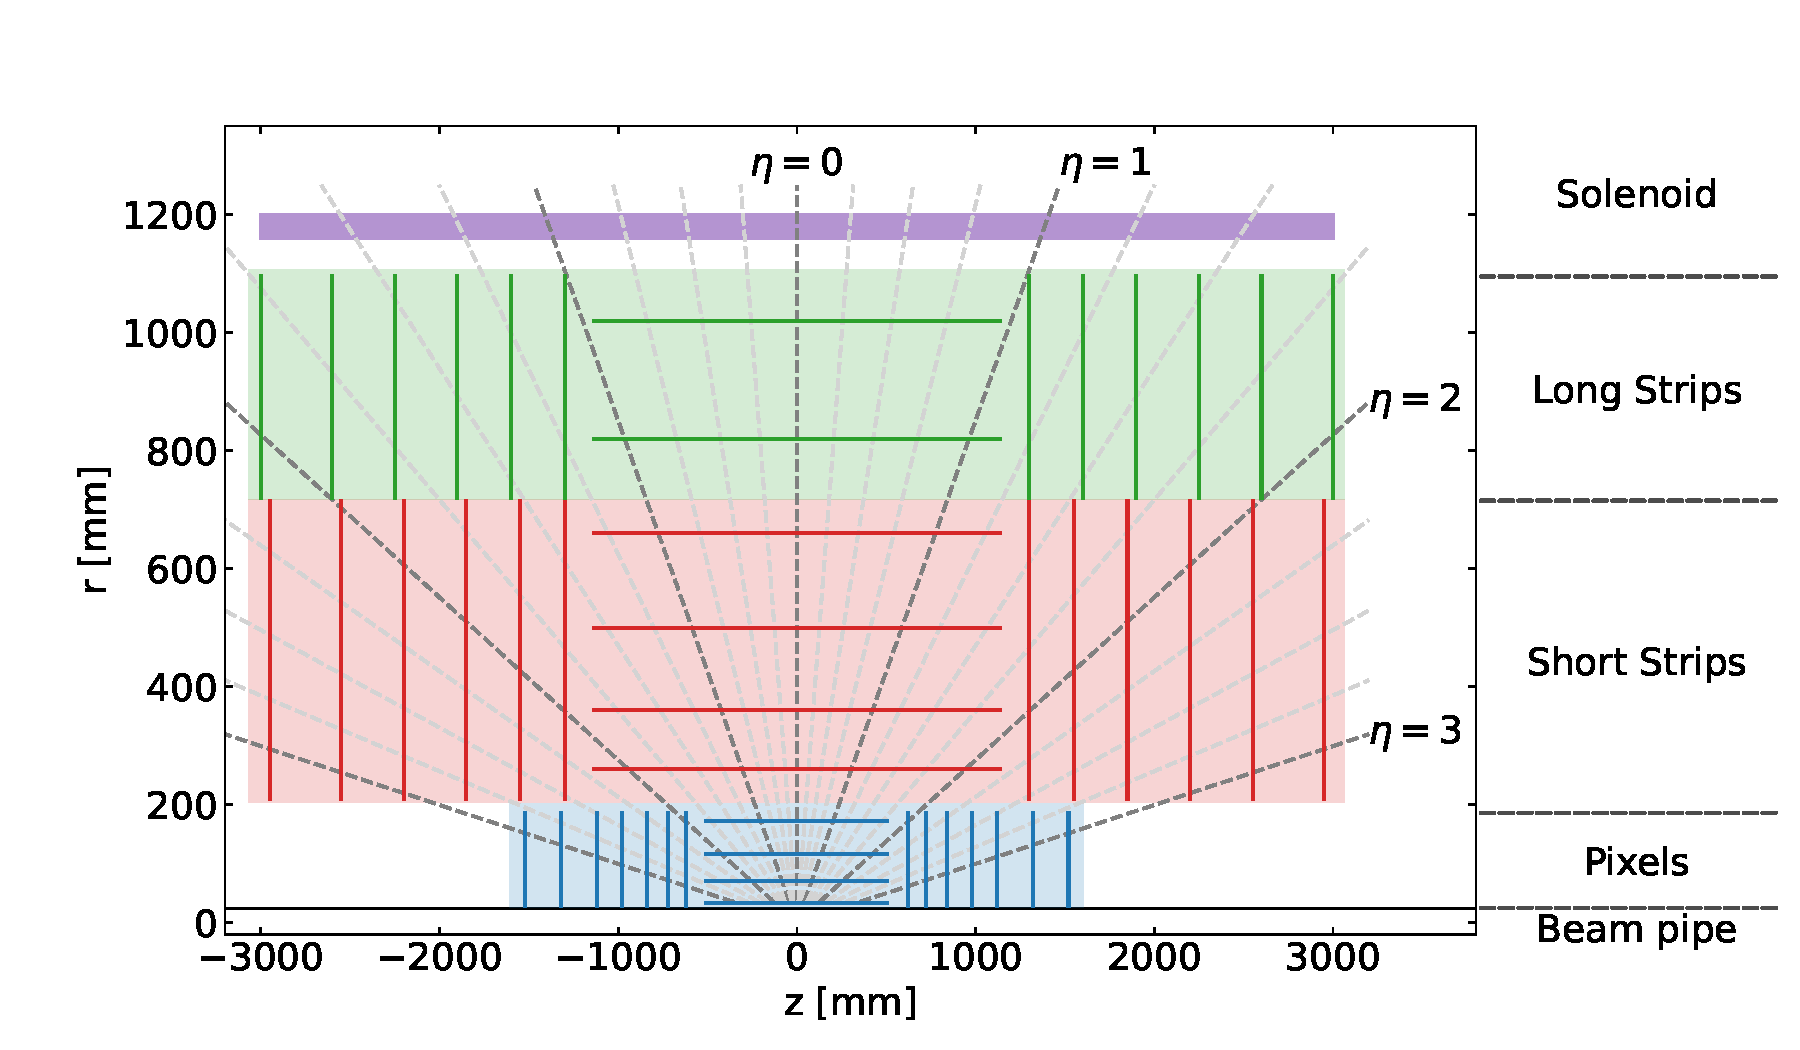
\includegraphics[width=0.6\linewidth]{figures/detector_layout.pdf}
  \caption{Visualization of the ODD layout segmented into Beam pipe, Pixels, Short Strips, Long Strips, and Solenoid. The solid lines inside the sub detectors represent the layers and disks. The dashed lines represent different eta regions.}
  \label{fig:odd_layout}
\end{figure}

\begin{table}[htb!]
    \centering
    \begin{tabular}{|c|c|c|c|}
       \hline
       \textbf{Sub detector} & \textbf{Measurement} & \textbf{Resolution} & \begin{tabular}{c}\textbf{\# Barrel Layers /}\\\textbf{\# Endcap Disks}\end{tabular} \\
       \hline
       Pixel & \begin{tabular}{c}2D\\(+time)\end{tabular} & \begin{tabular}{c}15 µm spatial\\(25 mm/c temporal)\end{tabular} & 4 / 7 \\
       \hline
       Short Strip & 2D & \begin{tabular}{c}43 µm spatial /\\1.2 mm spatial\end{tabular} & 4 / 6 \\
       \hline
       Long Strip & 1D & 72 µm spatial & 4 / 6 \\
       \hline
    \end{tabular}
    \caption{Details about the ODD sub detectors. Note that spatial and temporal resolutions are customizable but consistently used in an ACTS context, as here. Time components are put in parenthesis as they are considered optional.}
    \label{tab:odd_details}
\end{table}

The ACTS Examples Framework uses the ODD detector description by constructing a tracking geometry which allows for fast track simulation (ActsFatras\cite{acts}) and track reconstruction. A more realistic simulation can be achieved using Geant4 for full detector simulation. Events can be generated using a simple ACTS particle gun or Pythia8. The different steps of the simulation and reconstruction chain are placed into a \textit{Sequencer} object which executes the algorithms in the requested order. \textit{Readers} and \textit{Writers} can be used to persist data at every step in the sequence of algorithms.

%Figure \ref{fig:odd} shows the sensitive surfaces of the ODD after constructing the tracking geometry with the ACTS Examples Framework.
%
%\begin{figure}[htb!]
%  \centering
%  \includegraphics[width=0.9\linewidth]{figures/odd.png}
%  \caption{Illustration of the ODD and its sensitive surfaces of the 3 sub detectors: \textcolor{green}{Pixels}, \textcolor{orange}{Short Strips} and \textcolor{blue}{Long Strips}.}
%  \label{fig:odd}
%\end{figure}

The reference frame used for our detector is defined as follows: the Z axis points along the beam line, the Y axis points towards the center of an imaginary accelerator, and the X axis is determined by the right hand rule. The azimuthal angle $\phi$ is defined as $\text{atan2}\left(y,x\right)$ in the transverse plane XY and the polar angle $\theta$ is defined as $\text{atan2}\left(\sqrt{x^2+y^2},z\right)$. The pseudo rapidity $\eta$ is given by $-\ln\left[\tan\left(\frac{\theta}{2}\right)\right]$.

\section{Simulation and reconstruction chain}
\label{reco}

The simulation and reconstruction chain used to produce our results is the following:

\begin{itemize}
  \item The following events have been generated
    \begin{itemize}
      \item Single muon, pion, electron events with fixed transverse momentum of $p_T=1,10,100$ GeV and uniform pseudo rapidity $|\eta|<3$
      \item Single muon, pion, electron events with a uniform transverse momentum distribution $1 \text{GeV} < p_T < 100 \text{GeV}$ and uniform pseudo rapidity disribution $|\eta|<3$
      \item $t\overline{t}$ events with a center of mass energy $\sqrt{s} = 14$ TeV and average pileup\footnote{Pileup is the number of simultaneous collisions which are not relevant for a physics search e.g. soft scatter vs hard scatter vertices} $|\mu|=60,120,200$
    \end{itemize}
  \item The detector simulation is obtained using Geant4.%: DD4hep exports the ODD geometry description which is directly provided to Geant4. The default physics list \texttt{FTFP\_BERT} is used.
  \item A \textit{smeared digitization} approach is used to simulate the detector response. Simulated hit positions are smeared using Gaussian noise corresponding to the detector resolution shown in Table \ref{tab:odd_details}. These resolutions are also provided as cluster uncertainties to the fitters during reconstruction.
\end{itemize}

\begin{flushleft}
The simulation data is reconstructed using the following reconstruction chain:
\end{flushleft}

\begin{itemize}
  \item Seed finding provides a first estimation of the track parameters which is used as an input of the track finding. A truth based seeding was chosen for the studies presented in this document. The algorithm takes the true parameters of the particles at its origin in the beam pipe and applies a Gaussian noise.\footnote{In the ACTS context this is called \textit{truth smeared seeding}.}
  \item Track finding and fitting based on Combinatorial Kalman Filter (CKF)
  \item Ambiguity resolution algorithm to remove duplicated tracks based on clusters information realized with a greedy approach with cuts on a maximum number of shared hits on tracks.
\end{itemize}

\begin{figure}[htb!]
  \centering
  \begin{overpic}[width=0.7\linewidth,percent]{figures/ttbar_event.png}
    \put(3,57){\parbox{15em}{
      ODD Simulation\\
      $t\overline{t}$, $\langle\mu\rangle=200$\\
      $\sqrt{s} = 14$ TeV
    }}
  \end{overpic}
  \caption{Illustration of a $t\overline{t}$ event at $\langle\mu\rangle=200$. Hits of charged particles are displayed as red points and reconstructed tracks as white lines.}
  \label{fig:ttbar_event}
\end{figure}

\begin{flushleft}
Figure \ref{fig:ttbar_event} shows a $t\overline{t}$ event at $\langle\mu\rangle=200$ which was generated and reconstructed with the chain described above.
\end{flushleft}

\section{Key Performance Indicators}
\label{kpi}

Reconstructed tracks are matched to simulate particles to evaluate Key Performance Indicators (KPI). This is done by relating the measurements on track with the particles producing them and choosing a cut-off threshold that determines which track belongs to a certain particle.\cite{ATL-PHYS-PUB-2015-051}\cite{CERN-LHCC-2017-021} If multiple tracks correspond to the same particle (duplicate tracks), we select the one with the highest number of measurements and lowest $\chi^2$. Additionally, we define selection cuts on particles and tracks as follows:

\begin{itemize}
  \item Particles
    \begin{itemize}
      \item Originating from the primary vertex and within the beam pipe
      \item $p_T \ge 1$ GeV
      \item $|\eta| \le 3$
      \item \# hits $\geq 7$
      \item \# pixel hits $\geq 3$
      \item \# first pixel layer hits $\geq 1$
    \end{itemize}
  \item Tracks
    \begin{itemize}
      \item \# measurements $\geq 7$
      \item Truth matching cut-off: 50\%
    \end{itemize}
\end{itemize}

\begin{flushleft}
We define our KPIs as follows:
\end{flushleft}

\begin{itemize}
  \item Technical efficiency as a function of $\eta$ are defined as the ratio between the number of selected tracks to selected particles. Note that the requirement for the number of hits for the particles is restricting the sample to only reconstructible particles.\footnote{This requirement suppresses inefficiencies due to material interactions and is only useful to evaluate the performance of the track finding algorithm.}
  \item Track parameter resolutions are determined for the transverse impact parameter $d_0$ and the longitudinal impact parameter $z_0$ as a function of $\eta$ and $p_T$. For these parameters, the resolution is defined as the standard deviation of the residual between the true parameter value and the parameter value estimated from the track fitting as $\sigma(x_{\text{track}}-x_{\text{true}})$.
  \item Track parameter pulls are determined for the transverse impact parameter $d_0$, the longitudinal impact parameter $z_0$ and the ratio $\frac{q}{p}$ as a function of $\eta$. Track parameter pulls are defined as the ratio of the residual between the true parameter value and the parameter value estimated from the track fitting and the track parameter error estimate as $\frac{x_{\text{track}}-x_{\text{true}}}{\sigma_{\text{track}}}$.
\end{itemize}

\section{Impact parameter resolution}
\label{ip_res}

Figure \ref{fig:resolution_a} shows the impact parameter resolution for $d_0$ as a function of $\eta$ for single muons with $p_T = 1, 10, 100$ GeV. The resolution is determined by the spatial resolution of the innermost layers and the amount of material traversed by the particle, which is a function of $\eta$, $p_T$ and the magnetic field $B$. For high momentum particles, the resolution converges to the intrinsic resolution of 15 µm, determined by the spatial resolution of the innermost layer.

Figure \ref{fig:resolution_b} shows the impact parameter resolution for $z_0$ as a function of $p_T$ for single particles. The intrinsic resolution of 15 µm is approached at high $p_T$. We also observe a slightly worse resolution for electrons which is due to the Kalman filter not accounting for Bremsstrahlung. This  can be improved by using a Guassian Sum Filter (GSF) which is also available in ACTS but not shown for comparison in this work.\cite{acts_gsf}

\begin{figure}[htb!]
    \centering
    \def\captiona{$d_0$ resolution as a function of $\eta$ with $p_T = 1, 10, 100$ GeV for single muon events.}
    \subfloat[\captiona]{
        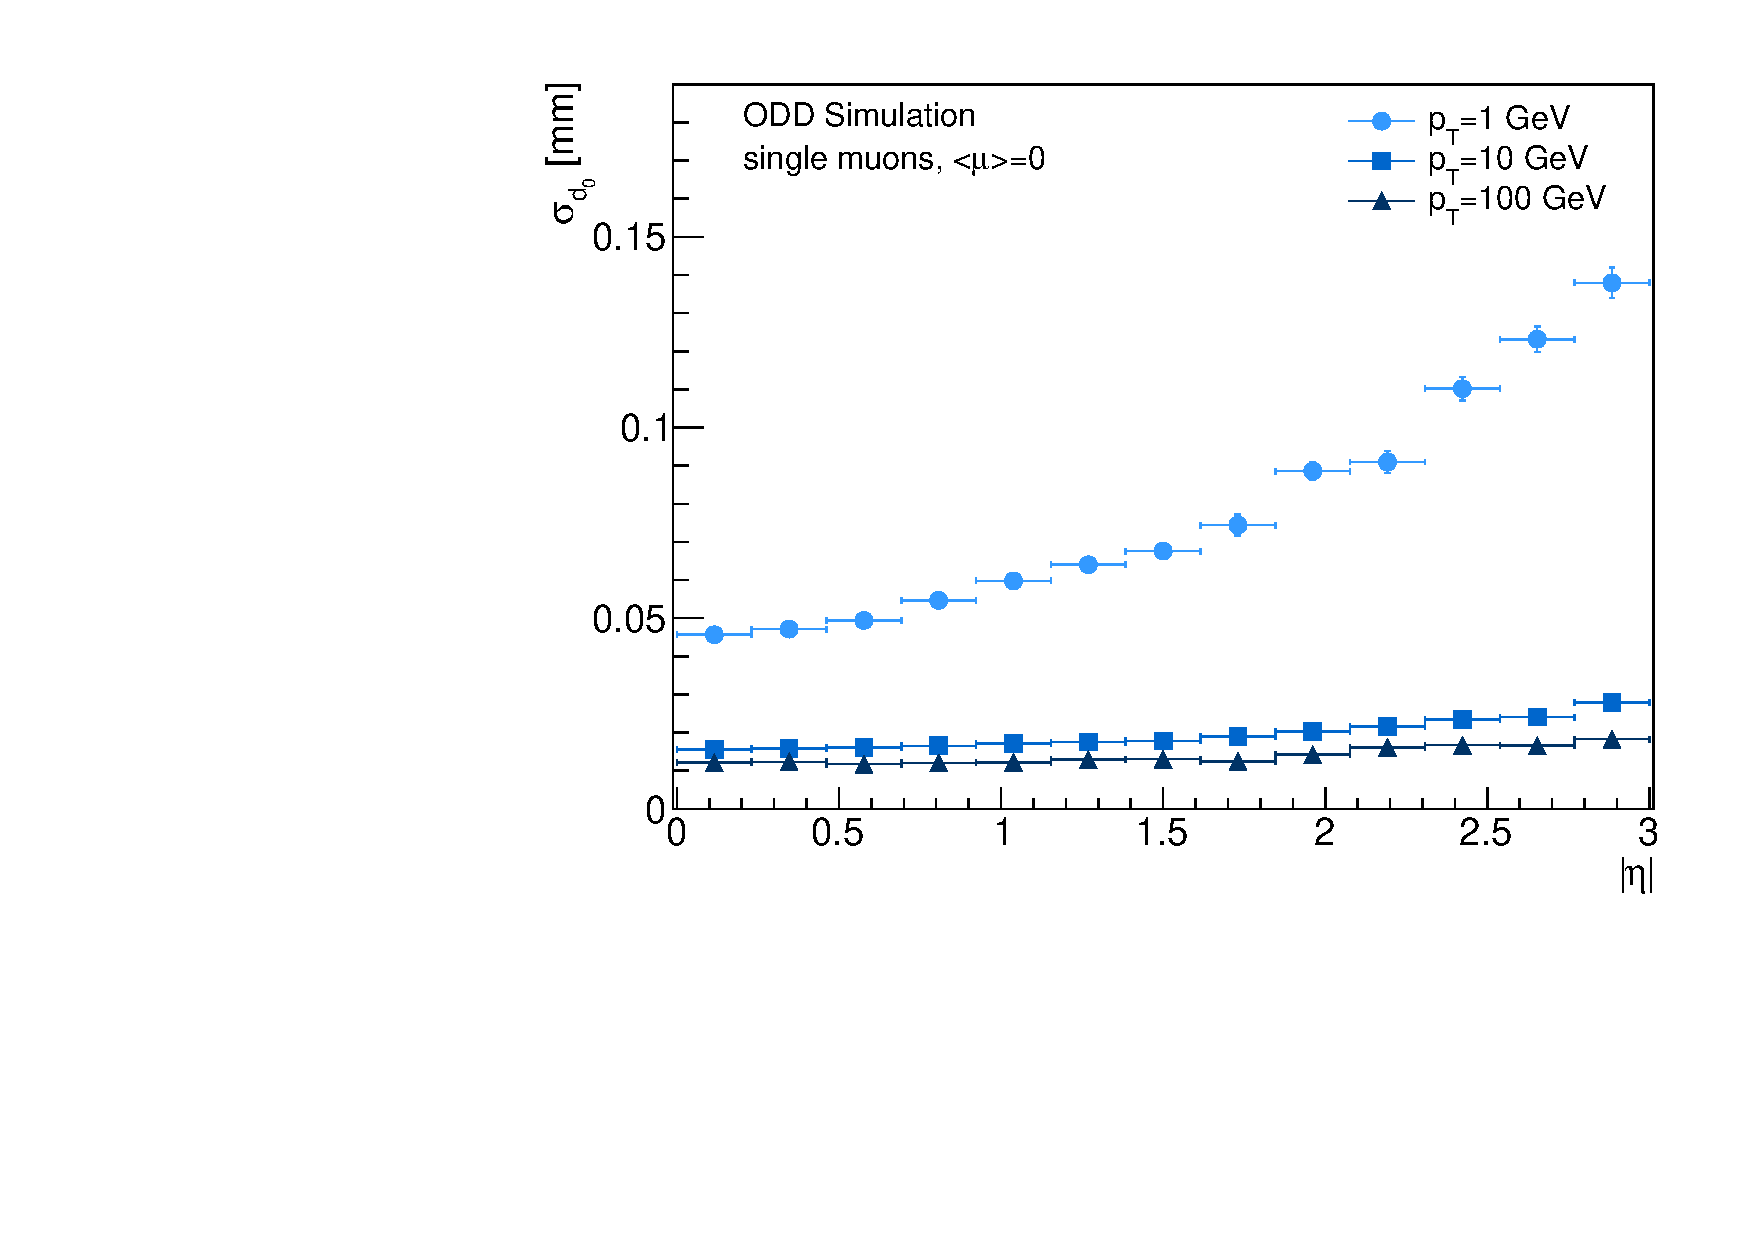
\includegraphics[width=0.45\linewidth]{figures/single_muon_resolution.pdf}
        \label{fig:resolution_a}
    }
    \qquad
    \def\captionb{$z_0$ resolution as a function of $p_T$ for single muon, pion and electron events.}
    \subfloat[\captionb]{
        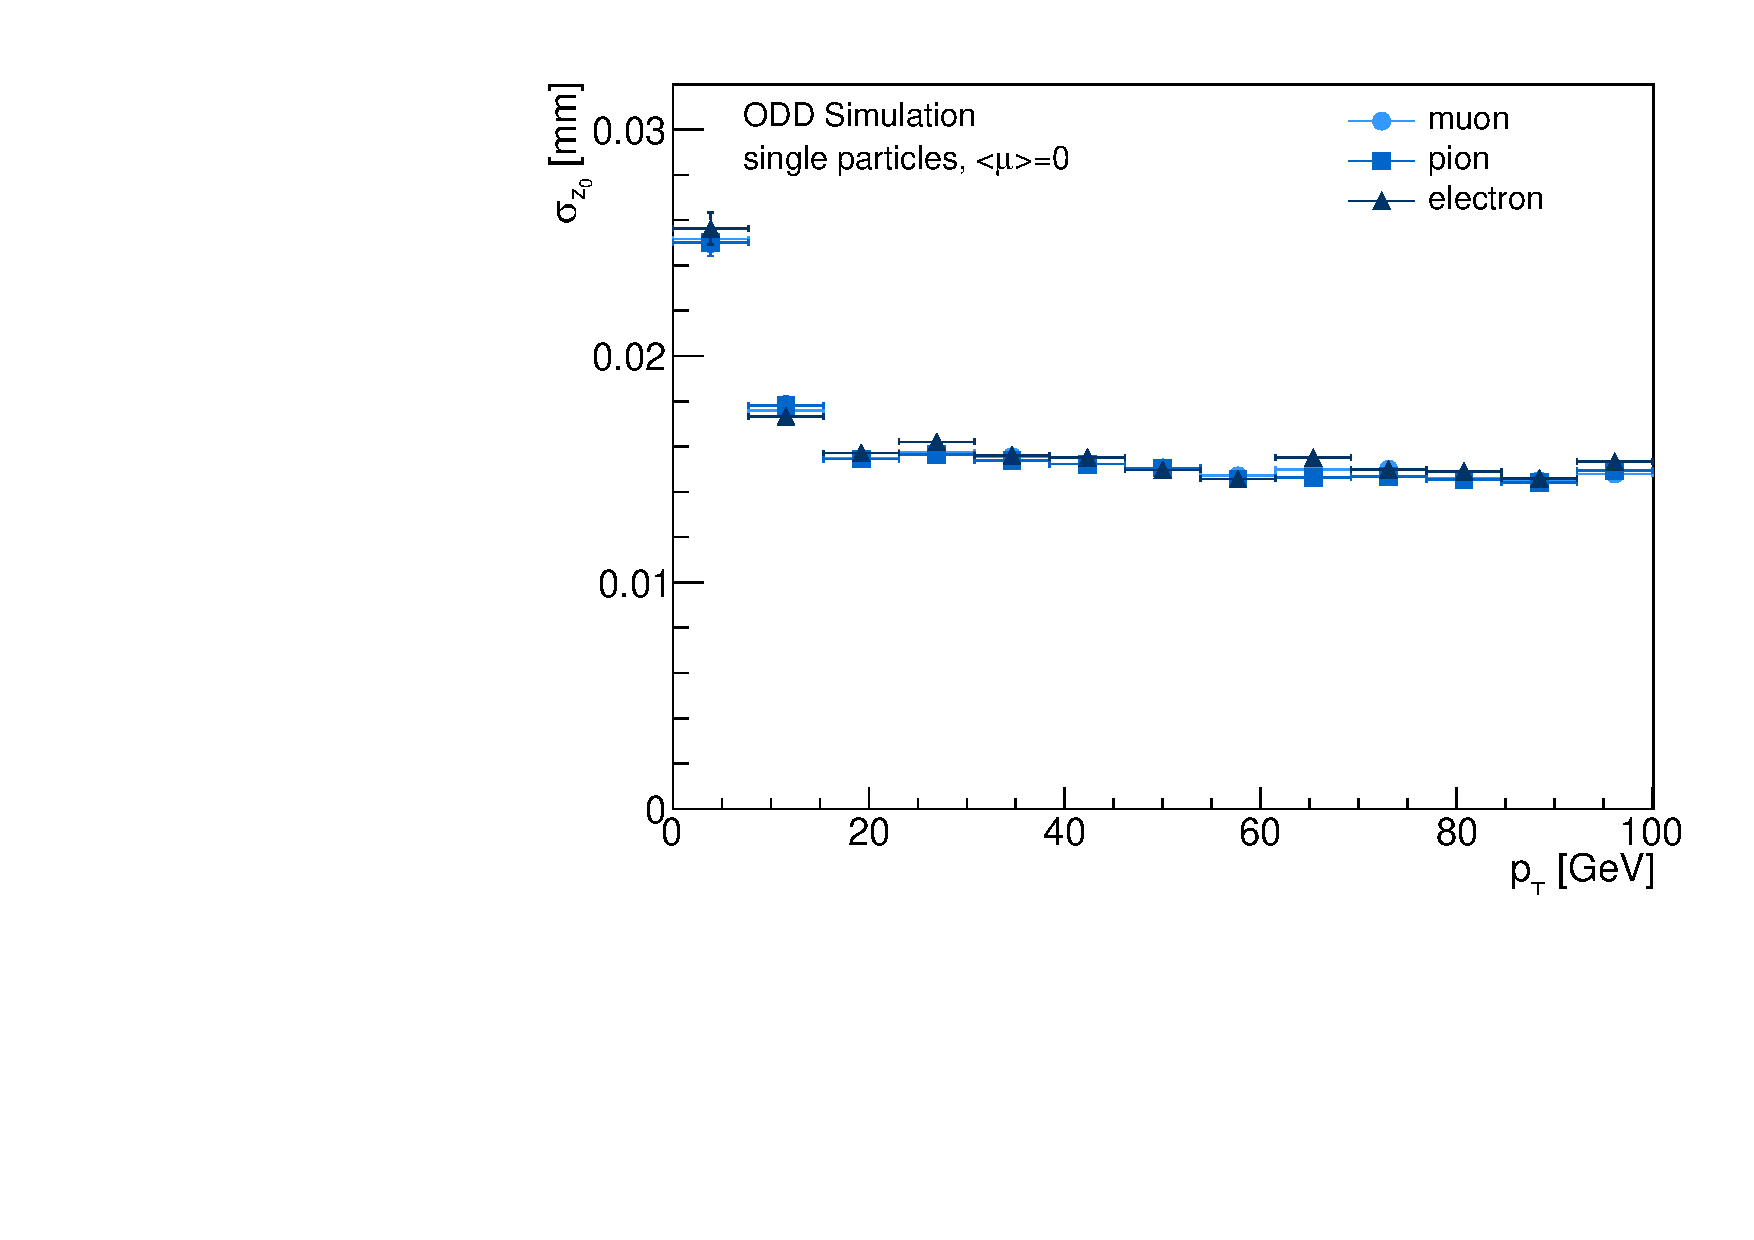
\includegraphics[width=0.45\linewidth]{figures/single_particle_resolution.pdf}
        \label{fig:resolution_b}
    }
    \caption{Resolution of (a) $d_0$ and (b) $z_0$ as a function of $\eta$ and $p_T$ for single particle events.}
    \label{fig:resolution}
\end{figure}

\section{Pulls}
\label{pulls}

%The pull is defined as the ratio of the residual and the error estimate for a given track parameter.
%\[\text{pull} = \frac{x^{\text{reco}} - x^{\text{true}}}{\sigma^{\text{reco}}}\]

Figure \ref{fig:pulls} shows the pulls of $d_0$, $z_0$ and $\frac{q}{p}$ for single muon events with $p_T=1,10,100$ GeV as a function of $\eta$. We observe good agreement with the ideal standard normal distribution $\mathcal{N}(0,1)$, which validates an unbiased covariance estimation of the track parameters.
%A small bias is observed at high $\eta$ and $p_T$ which is due to projection effects on the perigee surface.

\begin{figure}[htb!]
  \centering
  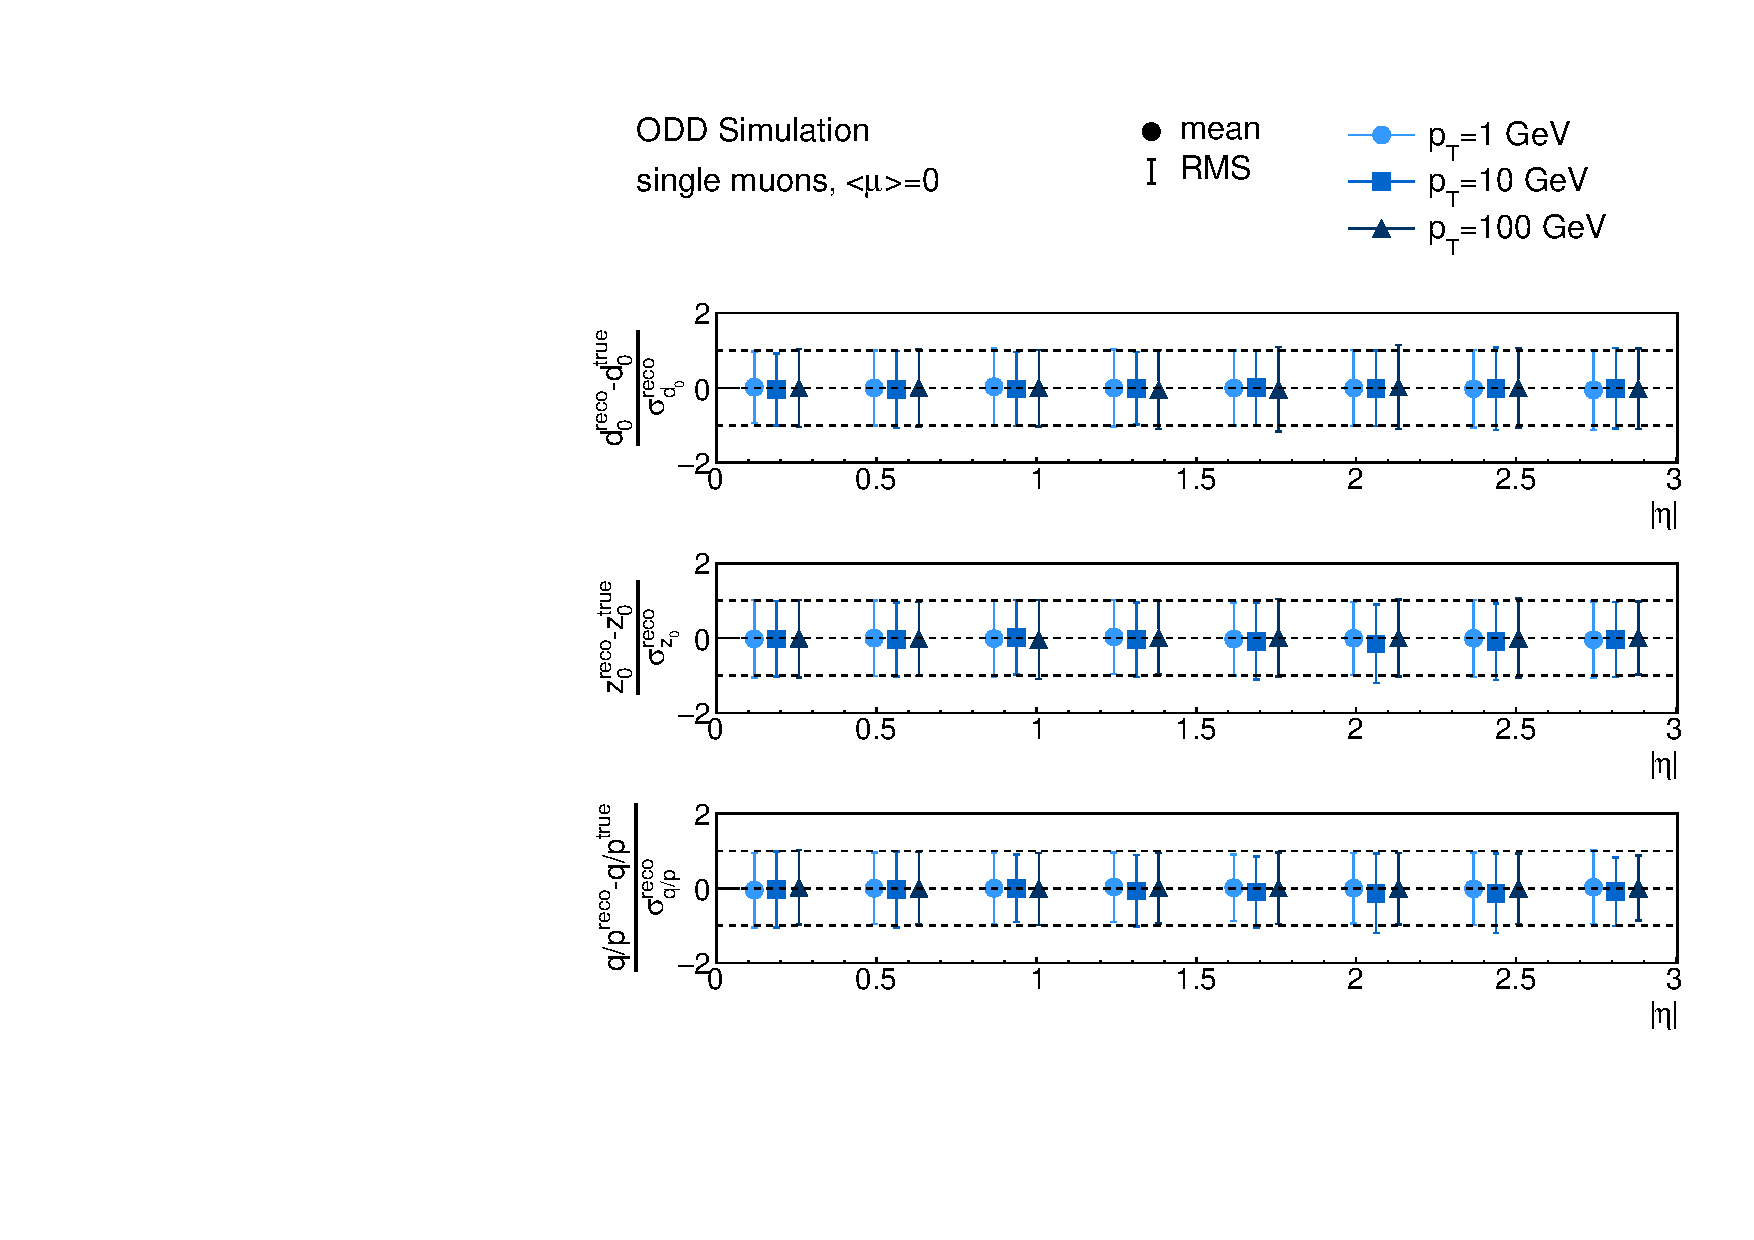
\includegraphics[width=0.6\linewidth]{figures/single_muon_pulls.pdf}
  \caption{Pulls of $d_0$, $z_0$ and $\frac{q}{p}$ for single muons with $p_T=1,10,100$ GeV as a function of $\eta$. The markers indicate the mean $\mu$ and the error bars the standard deviation $\sigma$ of a fitted $\mathcal{N}(\mu,\sigma)$ distribution. The dashed lines show the ideal values for these parameters.}
  \label{fig:pulls}
\end{figure}

\section{Technical efficiency for single particles}
\label{teff_single}

Single particle events provide an optimal scenario for a track finding algorithm as all hits in the detector are coming from that particle or secondaries produced by that particle. Therefore, studying the technical efficiency for such events provides an upper bound for any kind of physics event later on.

Figure \ref{fig:teff_single_a} shows the technical efficiency for single muons at $p_T=1,10,100$ GeV as a function of $\eta$. We observe efficiencies of about 99.9\% for $p_T=10,100$ GeV and $|\eta| < 2$. However for $p_T=1$ GeV we do not reconstruct more than $1\%$ of particles. Limitations of the ACTS CKF pattern recognition for low pT particles is currently under investigation.

Figure \ref{fig:teff_single_b} shows the technical efficiency for single muons, pions and electrons at $p_T=10$ GeV as a function of $\eta$. We observe efficiencies of about $99\%$ for pions and a drastic loss, up to $20\%$, for electrons. Improvements of the pattern recognition efficiency for electrons are currently under investigation.

\begin{figure}[htb!]
    \centering
    \def\captiona{single muon events with $p_T = 1, 10, 100$ GeV}
    \subfloat[\captiona]{
        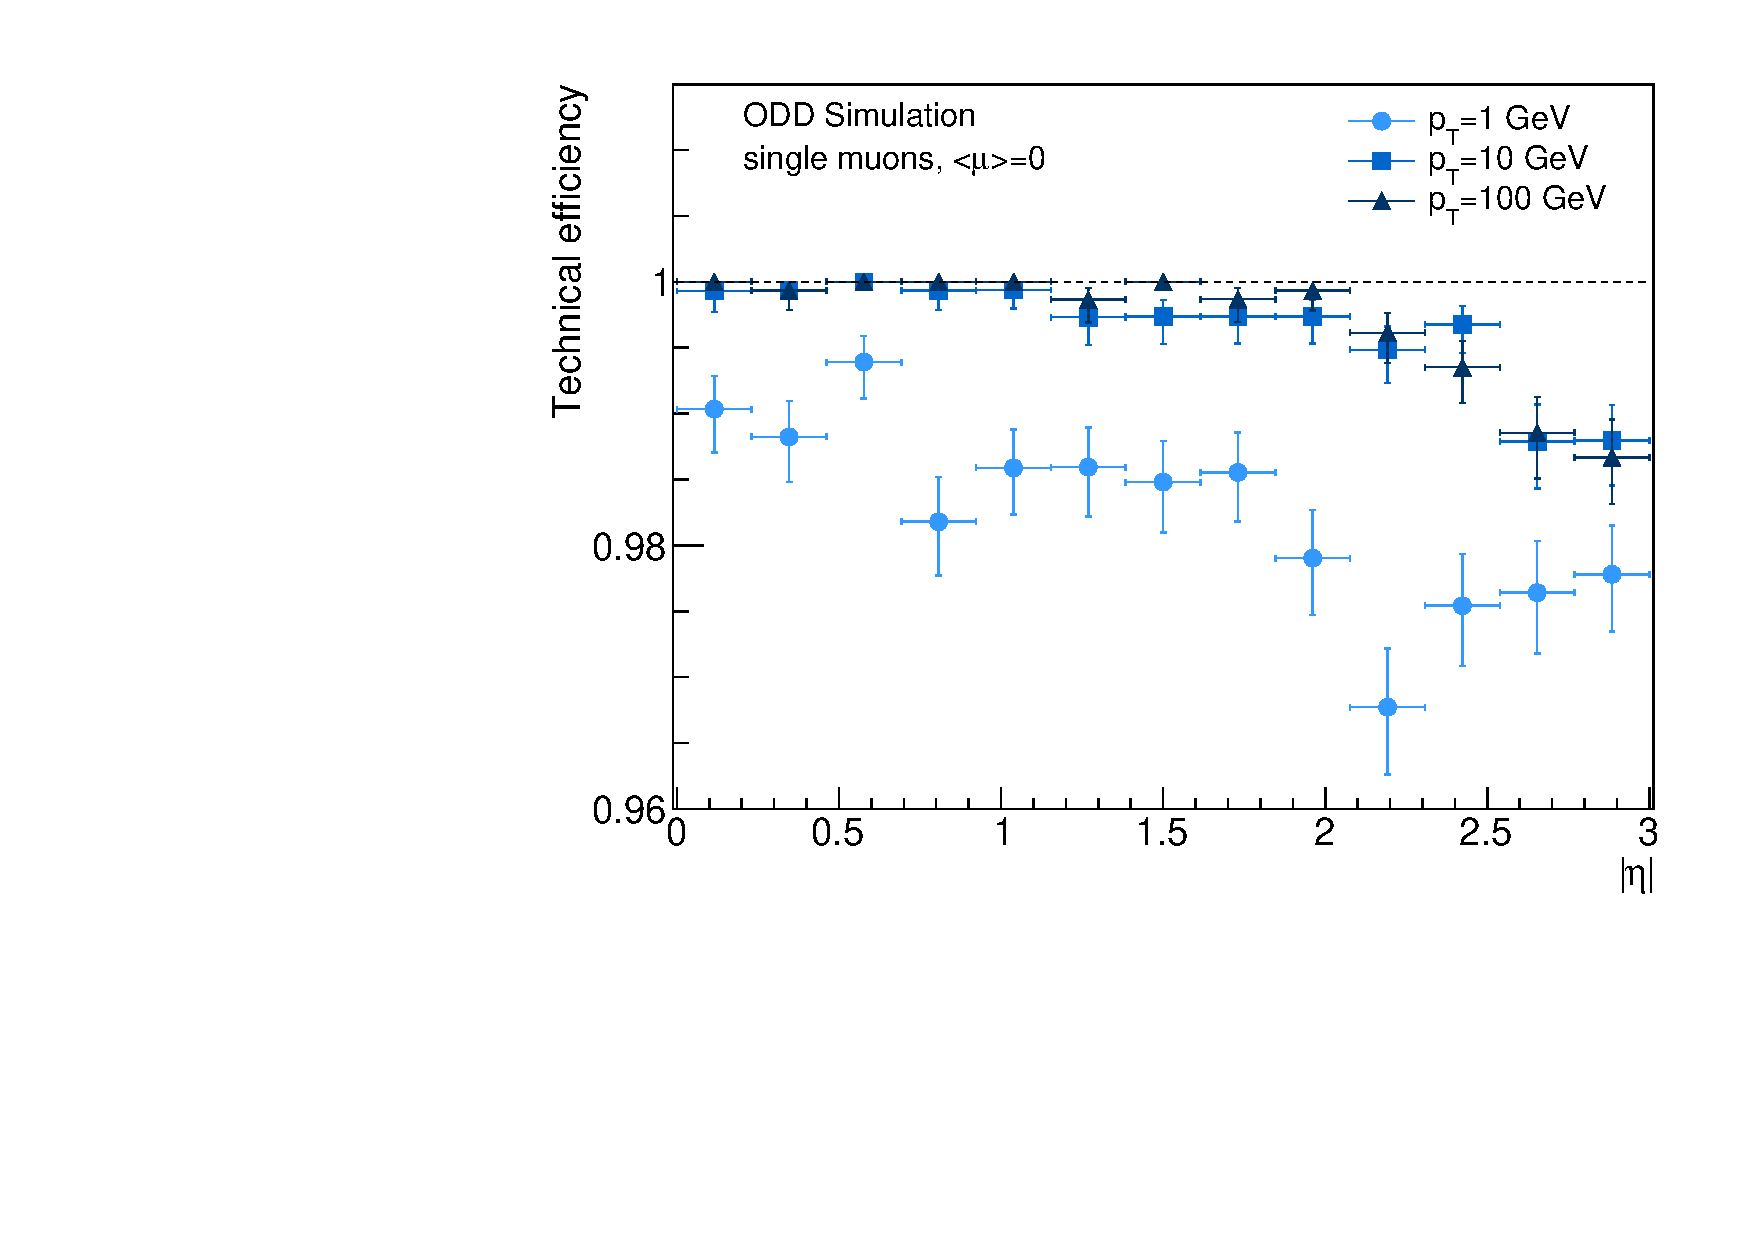
\includegraphics[width=0.45\linewidth]{figures/single_muon_efficiency.pdf}
        \label{fig:teff_single_a}
    }
    \qquad
    \def\captionb{single muon, pion, electron events with $p_T = 10$ GeV}
    \subfloat[\captionb]{
        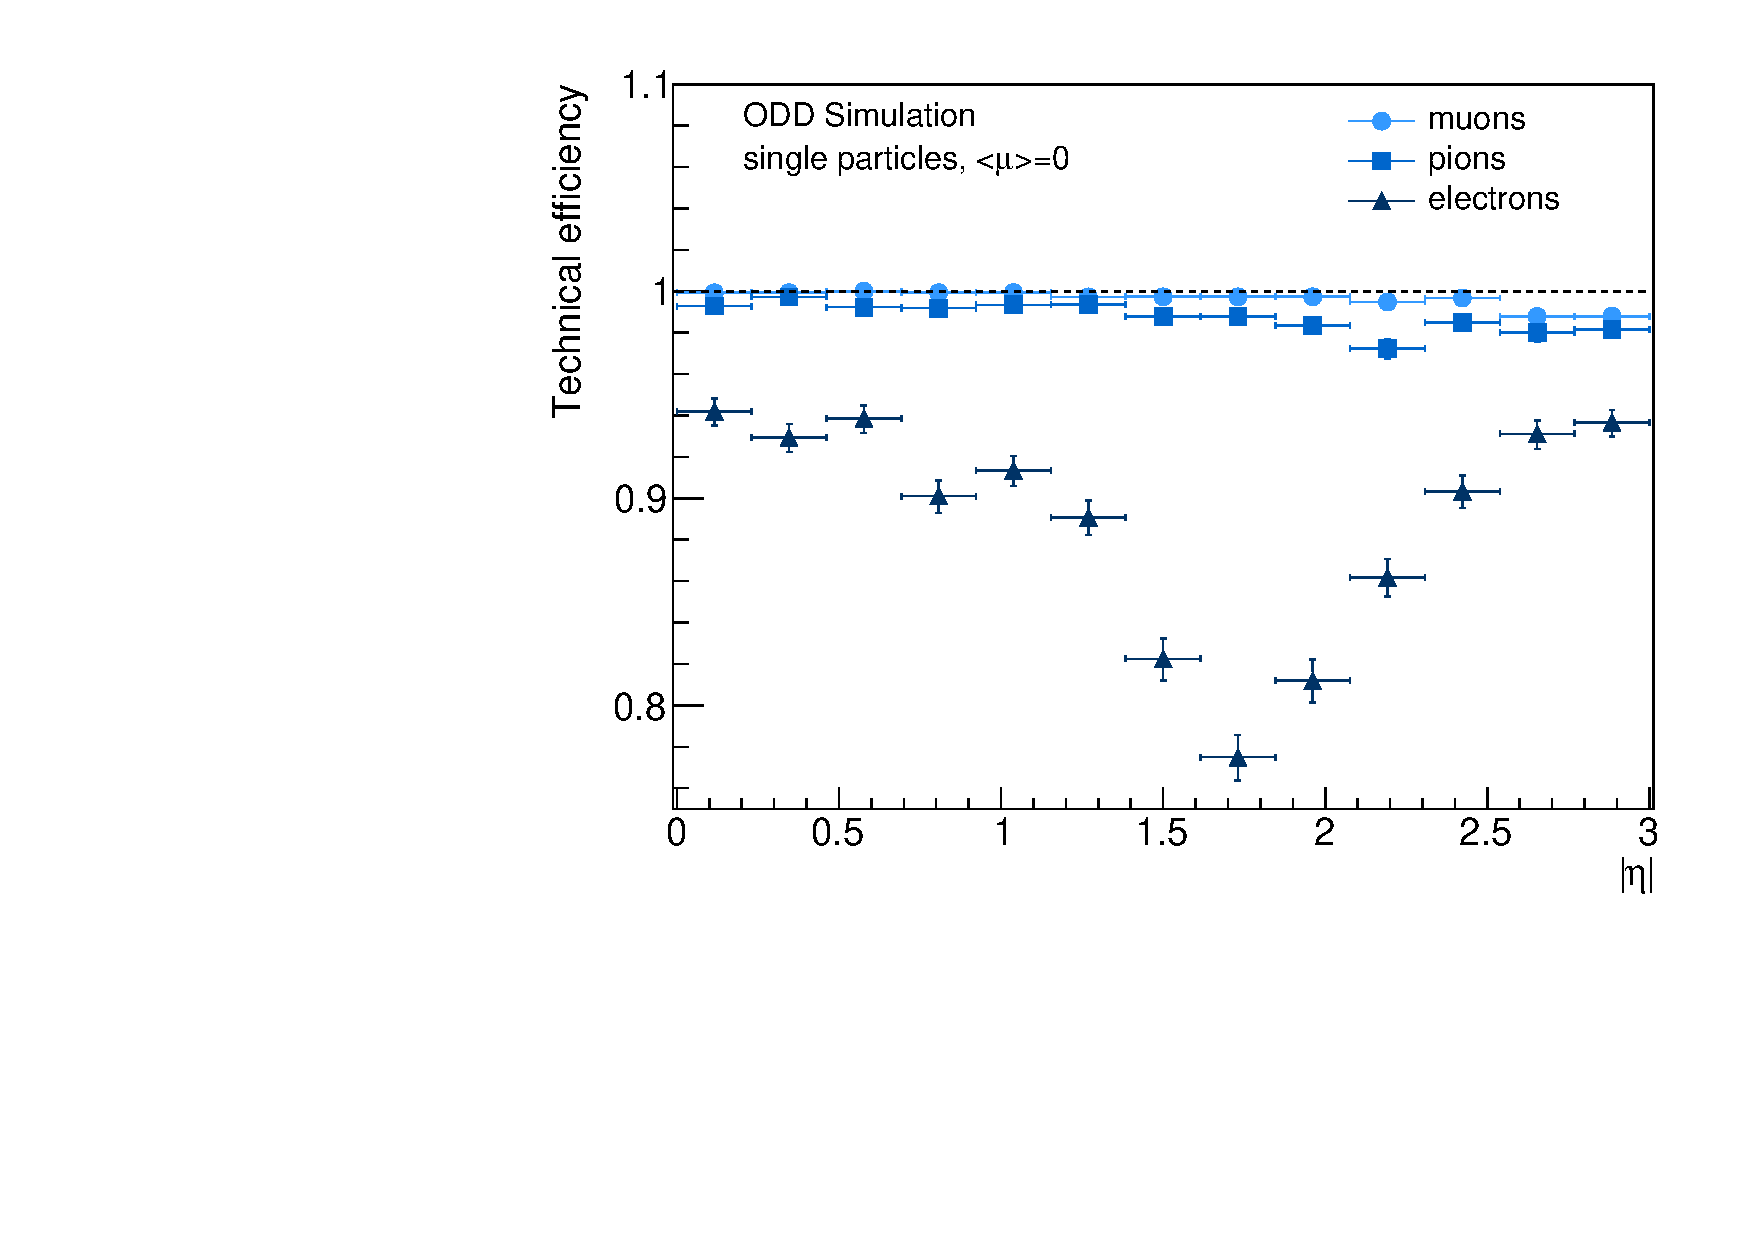
\includegraphics[width=0.45\linewidth]{figures/single_particle_efficiency.pdf}
        \label{fig:teff_single_b}
    }
    \caption{Technical efficiency for (a) single muons and (b) single particles as a function of $\eta$. The optimal value is indicated with a dashed line.}
    \label{fig:teff_single}
\end{figure}

\section{Technical efficiency for $t\overline{t}$}
\label{teff_ttbar}

A realistic scenario for a track finding algorithm in an LHC-like particle physics experiment is provided studying $t\overline{t}$ events at different $\langle\mu\rangle$ values, as effects of pattern recognition confusion and wrong hit assignments can affect tracking performance. For this study it was mainly used to measure the pileup dependency of the CKF.

Figure \ref{fig:teff_ttbar} shows the technical efficiency for $t\overline{t}$ events at $\langle\mu\rangle=60,120,200$ as a function of $\eta$. In case of \textit{truth smeared seeding} (Figure \ref{fig:teff_ttbar_a}) a severe pileup dependency is seen. This effect is strongly reduced if the \textit{truth smeared seeding} is replaced by the \textit{truth estimated seeding}, which builds track seeds from 3 pixel measurements for a given particle. This allows the track finding to start from the first measurement on the seed and therefore reduce combinatorics. The performance difference shows that the track finding can suffer in high occupancy environments when starting from the interaction point instead of the first measurement. 

%The truth \textit{estimated} seeding is another truth based seeder which forms a seed using 3 pixel measurements from one particle. In this case, the track finding will not start from the interaction point but from the first measurement which reduces combinatorics.

\begin{figure}[htb!]
    \centering
    \def\captiona{using truth \textit{smeared} seeding}
    \subfloat[\captiona]{
        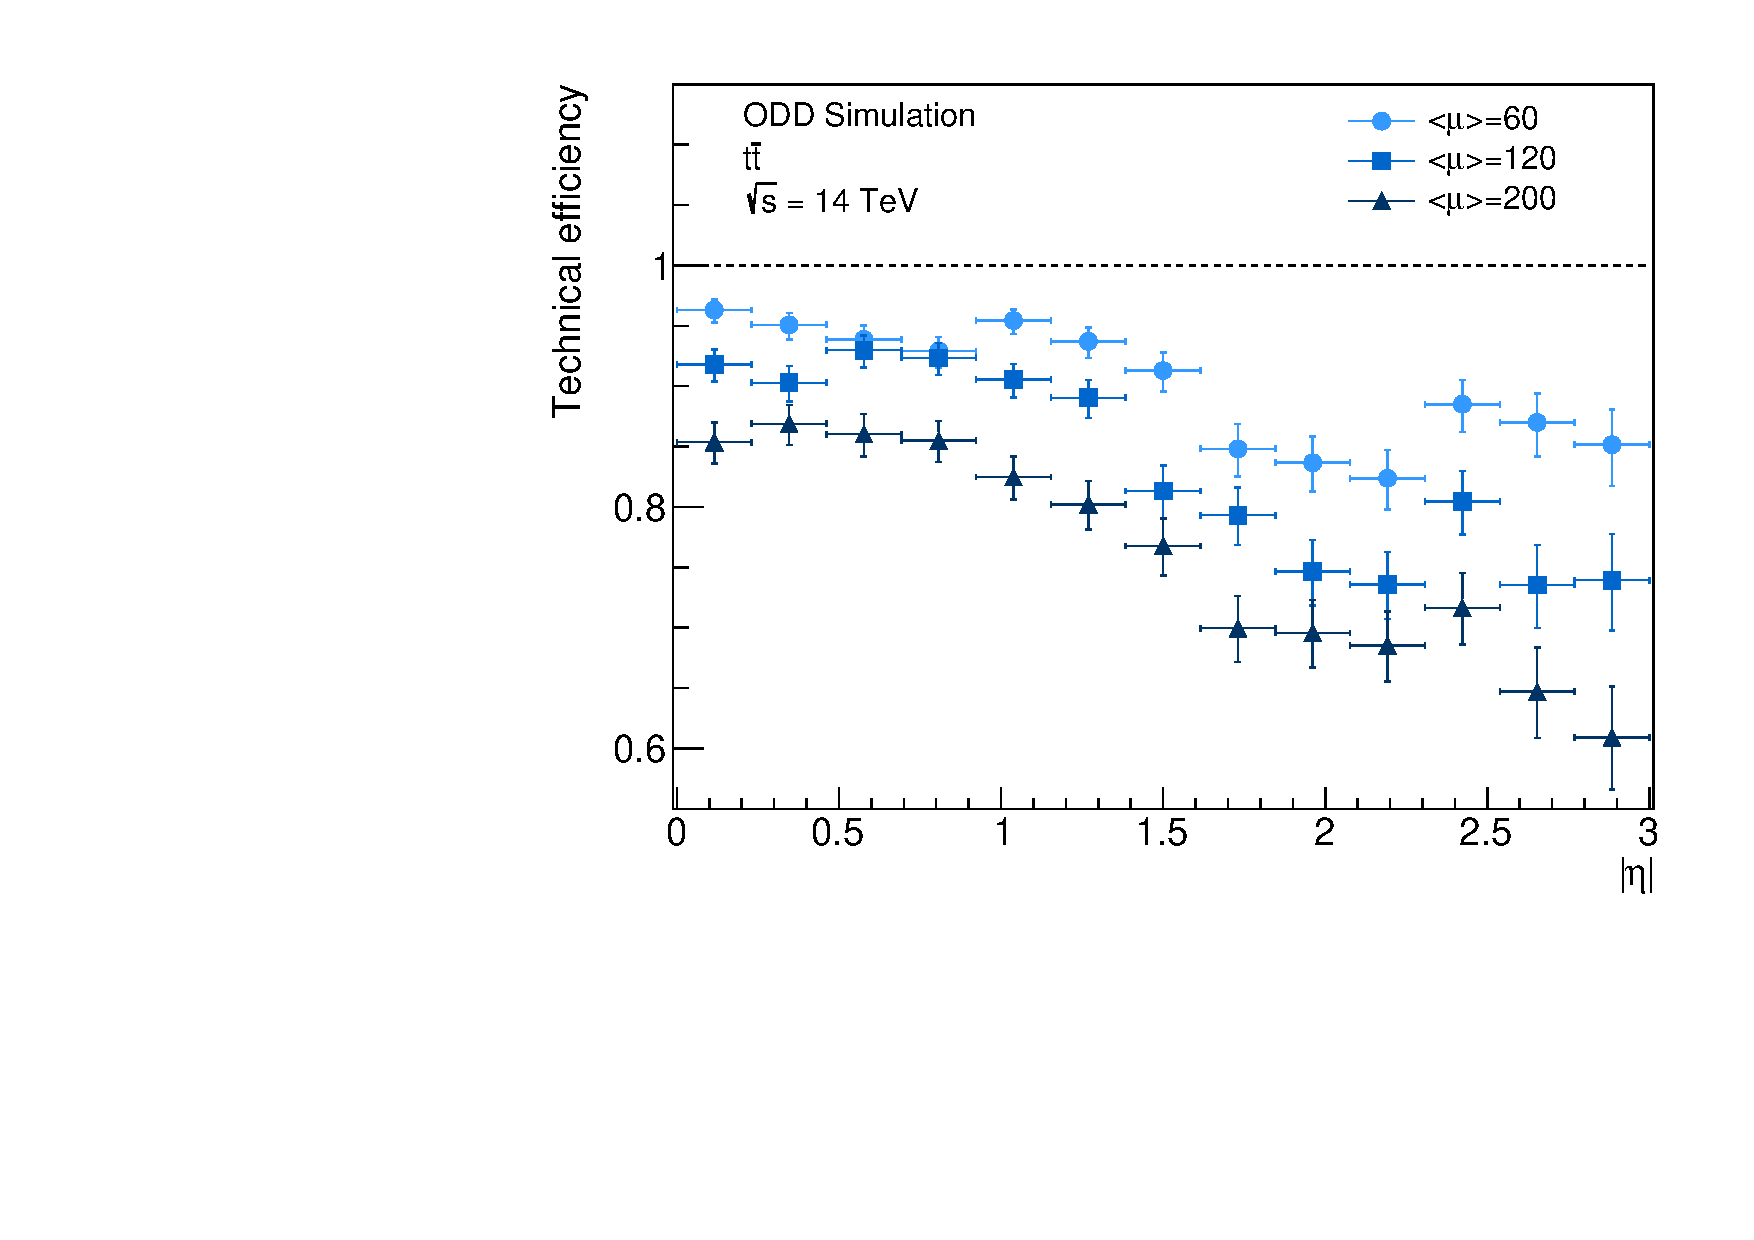
\includegraphics[width=0.45\linewidth]{figures/ttbar_efficiency_ts.pdf}
        \label{fig:teff_ttbar_a}
    }
    \qquad
    \def\captionb{using truth \textit{estimated} seeding}
    \subfloat[\captionb]{
        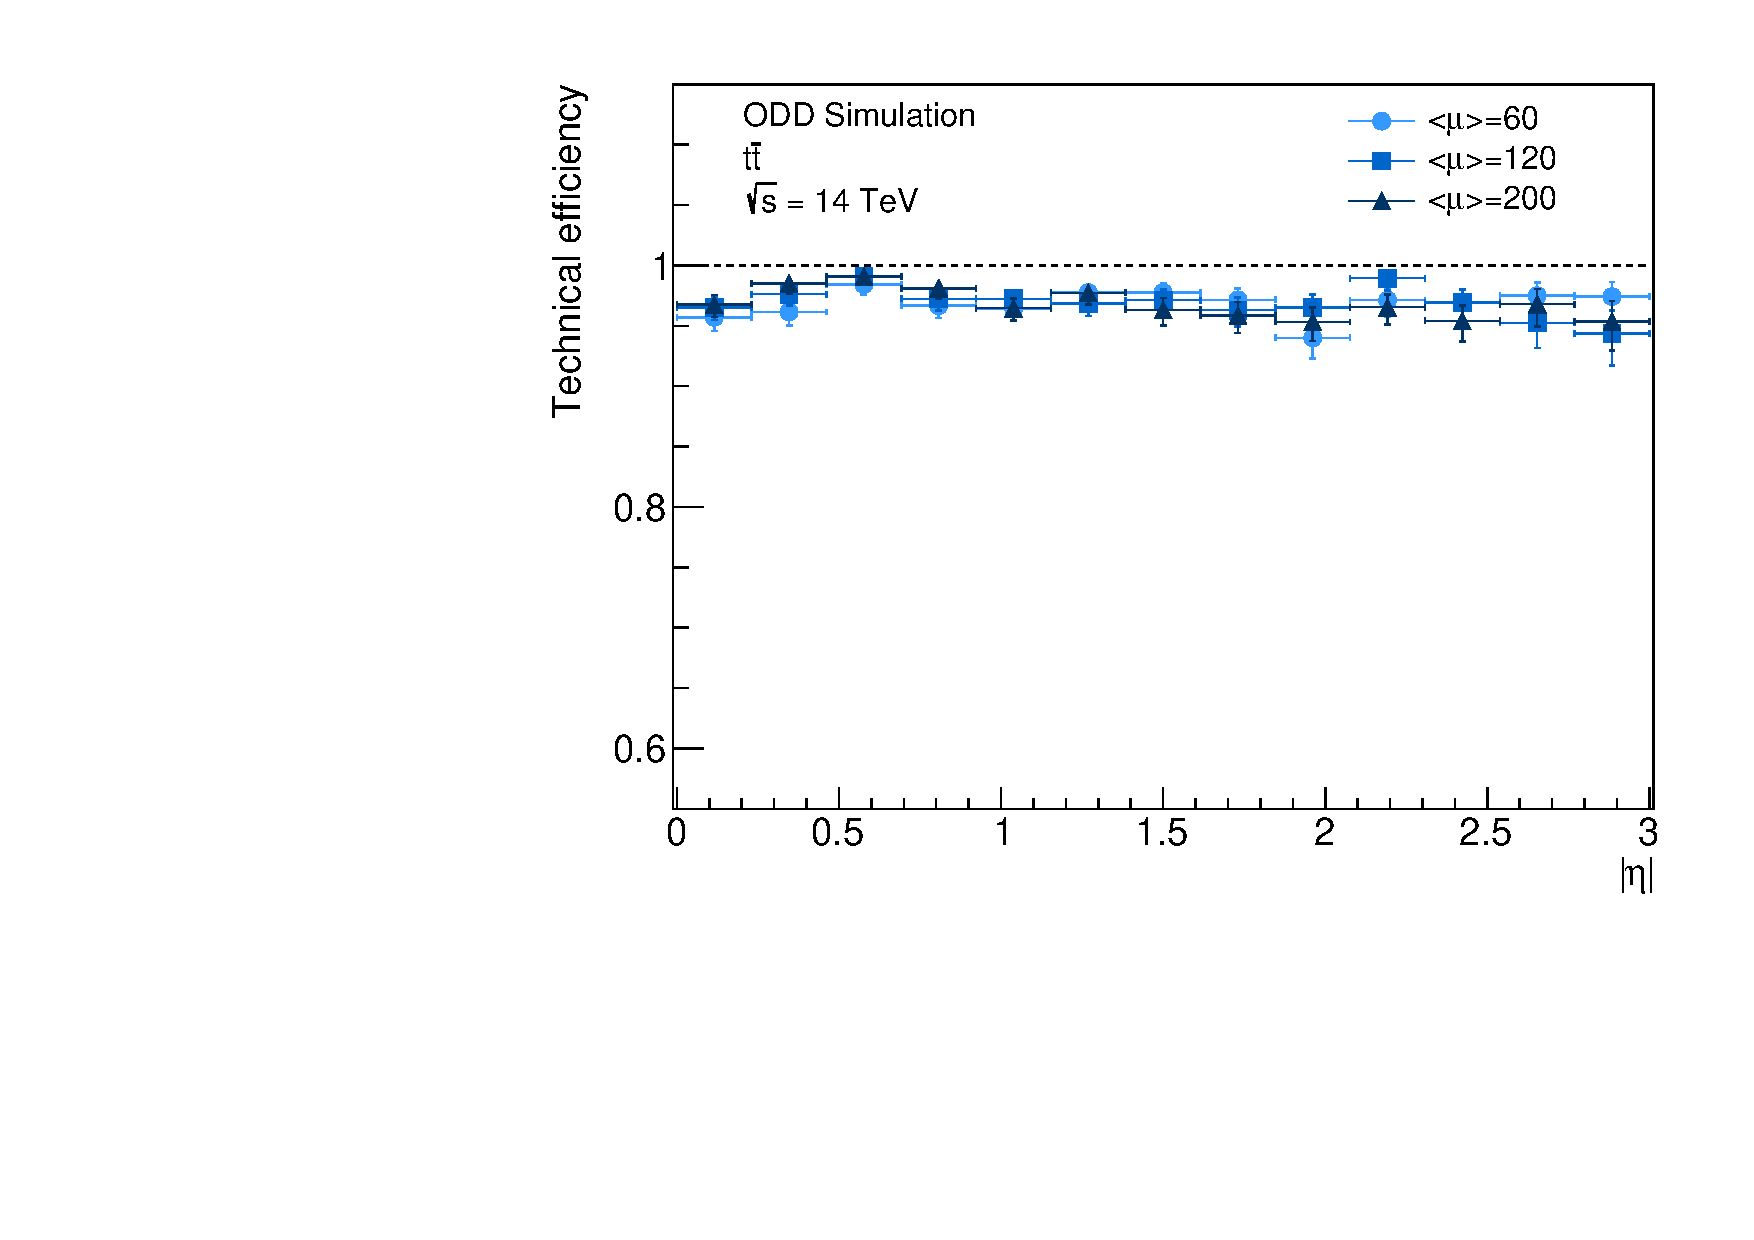
\includegraphics[width=0.45\linewidth]{figures/ttbar_efficiency_te.pdf}
        \label{fig:teff_ttbar_b}
    }
    \caption{Technical efficiency for $t\overline{t}$ events with $60, 120, 200$ for (a) \textit{truth smeared seeding} and (b) \textit{truth estimated seeding} pileup as a function of $\eta$. The optimal value is indicated with a dashed line.}
    \label{fig:teff_ttbar}
\end{figure}

%%%%%%%%%%%%%%%%%%%%%%%%%%%%%%%%%%%%%%%%%%%%%%%%%%%%%%%%%%%%%%%%%%%%%%%%%%%

\section{Conclusion}

With the presented work we have evaluated the current baseline track finding and fitting performance for the ODD using ACTS. The results show that material effects are very well under control as well as measurements uncertainties are handled correctly. This study provides an assessment of the current performance of the ACTS reconstruction chain using the ODD detector, showing that this framework is a viable R\&D platform for tracking algorithm research and detector prototyping.

This set of results has motivated further investigations in the ACTS pattern recognition components. Future plans and developments will investigate how to extend the studies towards a more realistic setup by enhancing the digitization and using a non-truth based seeder.

%%%%%%%%%%%%%%%%%%%%%%%%%%%%%%%%%%%%%%%%%%%%%%%%%%%%%%%%%%%%%%%%%%%%%%%%%%%  

%%  if necessary
%%\Acknowledgements
%%I am grateful to XYZ for fruitful discussions. Replace the text.

%%%%%%%%%%%%%%%%%%%%%%%%%%%%%%%%%%%%%%%%%%%%%%%%%%%%%%%%%%%%%%%%%%%%%%%%%%%

% TODO Am I allowd to use bibtex / biblatex?
\printbibliography

%%\begin{thebibliography}{99}

%%
%%  bibliographic items can be constructed using the LaTeX format in SPIRES:
%%    see    http://www.slac.stanford.edu/spires/hep/latex.html
%%  SPIRES will also supply the CITATION line information; please include it.
%%

%%\bibitem{example} 
%%  Author 1,
%%  "Article title,''
%%  Journal {\bf Volume}, Pages (Year)
%%  [arXiv:XXXX.YYYY [ZZZZ]].
%%
%%\end{thebibliography}

%%%%%%%%%%%%%%%%%%%%%%%%%%%%%%%%%%%%%%%%%%%%%%%%%%%%%%%%%%%%%%%%%%%%%%%%%%%

\end{document}
